	\newpage
\section{Określenie wymagań szczegółowych}		%2
%Dokładne określenie wymagań aplikacji (cel, zakres, dane wejściowe) – np. opisać przyciski, czujniki, wygląd layautu, wyświetlenie okienek. Opisać zachowanie aplikacji – co po kliknięciu, zdarzenia automatyczne. Opisać możliwość dalszego rozwoju oprogramowania. Opisać zachowania aplikacji w niepożądanych sytuacjach.

\subsection{Opis wymagań}

\hspace{1cm}Aplikacja korzystać będzie z czujnika GPS, który umożliwi pomiar pokonanej odległości oraz rzutowanie trasy na mapę - w tym celu użyte zostaną mapy Google. Na podstawie przebytej odległości będzie można określić także liczbę kroków oraz ilość spalonych kalorii. Odległości przebyte w poprzednich dniach będą zapisywane w aplikacji co pozwoli użytkownikowi na porównywanie swoich wyników z poszczególnych dni. W przypadku osiągnięcia wyniku poniżej wybranej normy użytkownik zostanie powiadomiony o tym fakcie przez aplikację. 
W celu zmiany motywu aplikacji użyty zostanie czujnik światła, dzięki któremu w trakcie dnia będzie funkcjonował tryb ciemny a w nocy tryb jasny. 
Użytkownik będzie miał możliwość zaznaczenia na mapie swojego celu, do którego chce danego dnia dotrzeć. Następnie będzie miał możliwość by przy użyciu aparatu w telefonie wykonać zdjęcie osiągniętego miejsca docelowego. Zdjęcie to będzie zapisywanie w folderze aparatu a użytkownik będzie miał wgląd w zdjęcia swoich poprzednich celów.
Aby ułatwić proces logowania Użytkownik będzie miał możliwość logowania do aplikacji za pomocą Facebook’a lub konta Google.
Aplikacja będzie działała cały czas bez potrzeby inicjowania. Możliwe będzie jej działanie w tle a także zwijanie do paska.

\subsection{Layout aplikacji}

\hspace{1cm}Na stronie głównej aplikacja będzie wyświetlać przebytą odległość, liczbę wykonanych kroków oraz liczbę spalonych kalorii. W prawym górnym rogu znajduje się przycisk, który po jego naciśnięciu umożliwi zalogowanie się do aplikacji. W lewym górnym rogu znajduje się przycisk otwierający menu.
	\begin{figure}[!htb]
		\begin{center}
				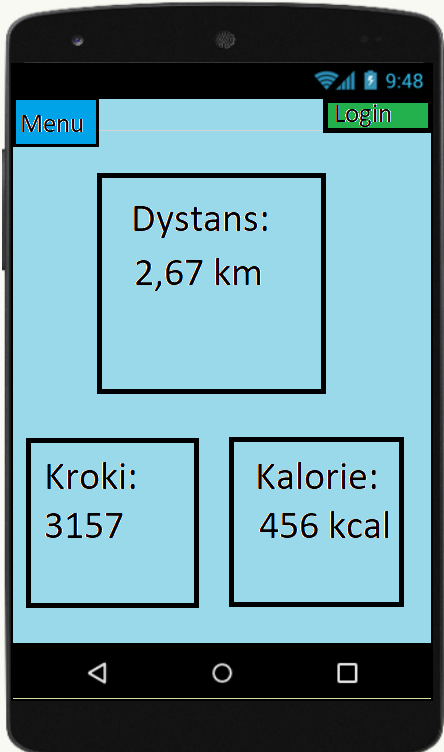
\includegraphics[width=3cm]{rys/Ap1.png}
				\caption{podstawowy layout aplikacji}
				\label{rys:rysunek001}
			\end{center}
	\end{figure}
\newline
Po otwarciu menu pojawi się lista w której znajdują się elementy takie jak: mapa - pokazuje przebytą trasę oraz umożliwia ustalenie swojego celu, wyniki - wyświetla wyniki osiągnięte w poprzednich dniach, Zdjęcia - otwiera galerię ze zdjęciami miejsc docelowych, wybierz normę - pozwala ustalić użytkownikowi jaki wynik chciałby osiągnąć.
\newline
  \begin{figure}[!htb]
	\begin{center}
		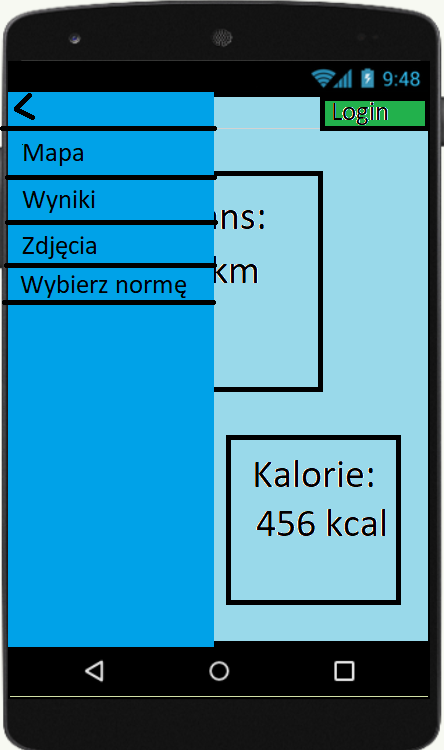
\includegraphics[width=3cm]{rys/Ap2.png}
		\caption{layout aplikacji po otwarciu menu}
		\label{rys:rysunek002}
	\end{center}
  \end{figure}






